
\section{Uncovering Microarchitecture via CPI Analysis}






\begin{frame}
    \frametitle{Uncovering Microarchitecture via CPI Analysis}
    \begin{block}{Problem: Hidden Microarchitecture}
        \begin{itemize}
            \item Internal details of CPU microarchitectures (e.g., pipelines, execution units, buffers) are often proprietary and not publicly documented in full detail.
            \item However, precise knowledge of these details is what allows mounting an effective side-channel attack
        \end{itemize}
    \end{block}
\end{frame}

\begin{frame}
    \frametitle{Uncovering Microarchitecture via CPI Analysis}
    \begin{block}{Inferring from CPI}
        \begin{itemize}
            \item A novel method is proposed: using information leaked by the \textbf{Clock cycles Per Instruction (CPI)} achieved on specific instruction sequences.
            \item \textbf{How it works}:
                \begin{itemize}
                    \item Compare CPI of instruction sequences with and without \textit{Read-After-Write (RAW) hazards}.
                    \item Hazard-free sequences reveal best-case CPU capabilities (e.g., dual-issuing).
                    \item Hazard-affected sequences show how hazards prevent parallel execution.
                \end{itemize}
            \item \textbf{Key Interpretations:}
                \begin{itemize}
                    \item A CPI of \textbf{0.5} indicates \textbf{full dual-issuing} (2 instructions per cycle).
                    \item A sustained CPI of \textbf{1} implies a component is \textbf{fully pipelined} (can start a new operation every cycle).
                \end{itemize}
        \end{itemize}
    \end{block}
\end{frame}

\begin{frame}
    \frametitle{Example: ARM Cortex-A7 MPCore}
    \begin{block}{CPU Overview}
        \begin{itemize}
            \item A dual-core, in-order CPU with an 8-stage pipeline.
            \item Described as "partial dual-issue": Not all instruction pairs can be executed simultaneously.
        \end{itemize}
    \end{block}

    \begin{block}{Why Characterize This CPU?}
        \begin{itemize}
            \item Public documentation (reference manuals, GCC backend descriptions) provides a logical view (see next slide).
            \item However, it lacks some microarchitectural details needed for side-channel analysis
        \end{itemize}
    \end{block}
\end{frame}


\begin{frame}
    \frametitle{ARM Cortex-A7 Pipeline Logical View}
    \begin{figure}
        \centering
        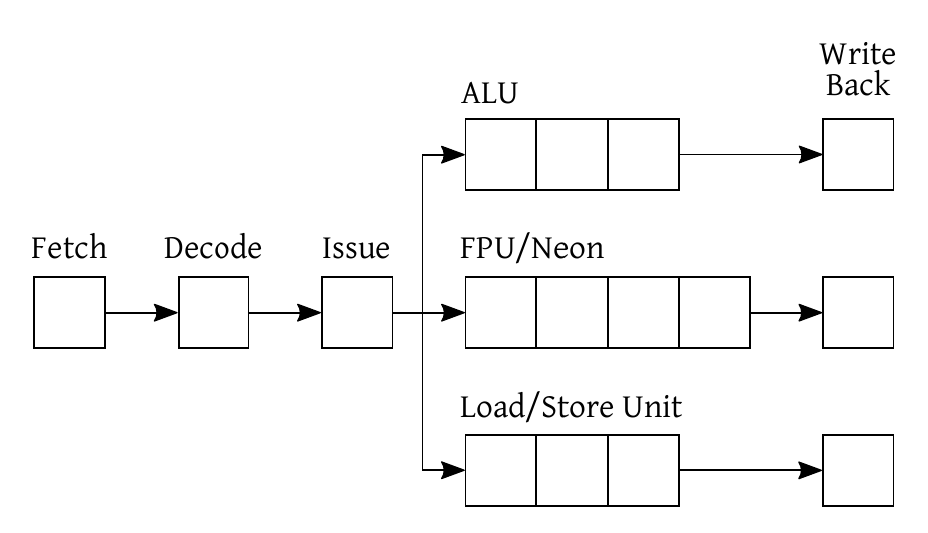
\includegraphics[width=0.8\textwidth]{Pictures/cortexA7.png} 
        \caption{ARM Cortex-A7 MPcore pipeline logical view }
        \label{fig:cortex-a7-pipeline}
    \end{figure}
\end{frame}


\begin{frame}
    \frametitle{Undercovering Microarchitectures (Cortex-A7 Example)}
    \begin{block}{Inferences from CPI Analysis}
        \begin{itemize}
            \item \textbf{ALUs:} Two ALUs are present, but they are not identical. Only one is equipped with a barrel shifter and multiplication unit.
            \item \textbf{Pipelined Units:}
                \begin{itemize}
                    \item The \textbf{Load Store Unit (LSU)} is \textbf{fully pipelined} (sustained CPI of 1 for load/store sequences).
                    \item The \textbf{multiplier} within the ALU is also \textbf{fully pipelined} (CPI of 1 for multiplication sequences).
                \end{itemize}
            \item \textbf{Data Bus Structure:}
                \begin{itemize}
                    \item Three data buses connect the Register File (RF) to the Execution (EX) stage.
                    \item Two buses connect the EX stage back to the RF, implying the RF has two write-ports and three read-ports.
                \end{itemize}
            \item \textbf{Unexpected NOP Behavior:} Counter-intuitively, \texttt{nop} instructions are \textbf{not dual-issued} by the Cortex-A7.
        \end{itemize}
    \end{block}
\end{frame}



\begin{frame}
    \frametitle{Deduction: Cortex-A7 Pipeline Structure}
    \begin{figure}
        \centering
        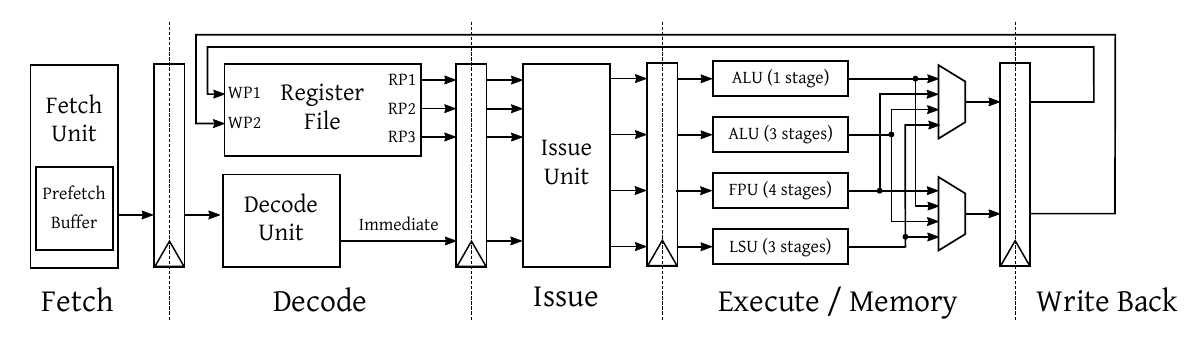
\includegraphics[width=1.0\textwidth]{Pictures/cortexUncovered.png}
        \caption{Alleged ARM Cortex-A7 pipeline structure according to CPI analysis deductions }
        \label{fig:deduced-pipeline}
    \end{figure}
\end{frame}



\begin{frame}
    \frametitle{Dual-Issue Capabilities: Instruction Pairs}
    \begin{table}
        \centering
        \small % makes the content of the table smaller
        \caption{Instruction pairs executed in dual-issue by the Cortex-A7 MPCore CPU. }
        \label{tab:dual-issue-pairs}
        \begin{tabular}{|l|c|c|c|c|c|c|c|}
            \hline
            \textbf{} & \textbf{mov} & \textbf{ALU} & \textbf{ALU w/imm} & \textbf{mul} & \textbf{shifts} & \textbf{branch} & \textbf{ld/st} \\
            \hline
            \textbf{mov}        & \checkmark & \checkmark & \checkmark & \ding{55} & \checkmark & \checkmark & \ding{55} \\
            \textbf{ALU}        & \checkmark & \ding{55}  & \checkmark & \ding{55} & \ding{55}  & \checkmark & \ding{55} \\
            \textbf{ALU w/ imm} & \checkmark & \checkmark & \checkmark & \ding{55} & \checkmark & \checkmark & \checkmark \\
            \textbf{branch}     & \checkmark & \checkmark & \checkmark & \checkmark & \checkmark & \ding{55}  & \checkmark \\
            \textbf{ld/st}      & \checkmark & \ding{55}  & \checkmark & \ding{55} & \ding{55}  & \checkmark & \ding{55} \\
            \textbf{mul}        & \ding{55}  & \ding{55}  & \ding{55}  & \ding{55} & \ding{55}  & \checkmark & \ding{55} \\
            \textbf{shifts}     & \ding{55}  & \ding{55}  & \checkmark & \ding{55} & \ding{55}  & \checkmark & \ding{55} \\
            \hline
        \end{tabular}
    \end{table}
\end{frame}